\section{PSR-Louvain and PH-Louvain}\label{GPUalg}
In this chapter, we present two novel parallel implementations of the Louvain algorithm: both versions implement the pruning presented by Ozaki et. al. \cite{pruning}.  The two algorithm differ on the way in which they accumulate the edges to calculate $l_{i\rightarrow C_j}$  (see formula \ref{ModularityC}). The first one, the PSR-Louvain, where PSR stands for Prune, Sort and Reduce Louvain, is based on the sort-reduce pattern: it sorts the list and performs a reduction of consecutive values with the same key. We also use a reduction on a sorted array to compute the maximum values of modularity for each node. 
The second algorithm, PH-Louvain, where PH stands for Prune and Hashmap Louvain, uses a map to accumulate that values.
In this chapter, we present firstly the algorithms, then a special speed-up technique of the first iteration of the optimization phase included in both algorithms and finally the data structure and the implementations details.

\subsection{PSR-Louvain}\label{Prune-Sort-Reduce}
The Prune, Sort and Reduce Louvain algorithm is the first version of the algorithm that we present in this thesis. As the sequential Louvain algorithm, we can divide it into two steps iterated alternately: the optimization phase and the aggregation phase. 
Furthermore, we divide the optimization phase in eight sub-phases, in which the operations are executed in parallel.
This algorithm takes in input a graph stored as a list of edges, where each entry is a tuple $(i,j,w)$: $i$ is the source node, $j$ is the destination node and $w$ is the weight of the edge; in this algorithm, even if the graph is undirected, we consider every edge twice reverting the order of the source and the destination. This list is sorted by $(i,j)$. In the beginning, we have each node is assigned to a community composed only by itself.
The weight of each node, a map that associate at each nodes the corresponding communities and the total weight of each communities. At the first iteration each node is in a community by itself and the total weight of each community corresponding at the weight of the unique node in it. The sub-phases of the optimization phase are the following:\\
\begin{figure}[t!]
	\centering
	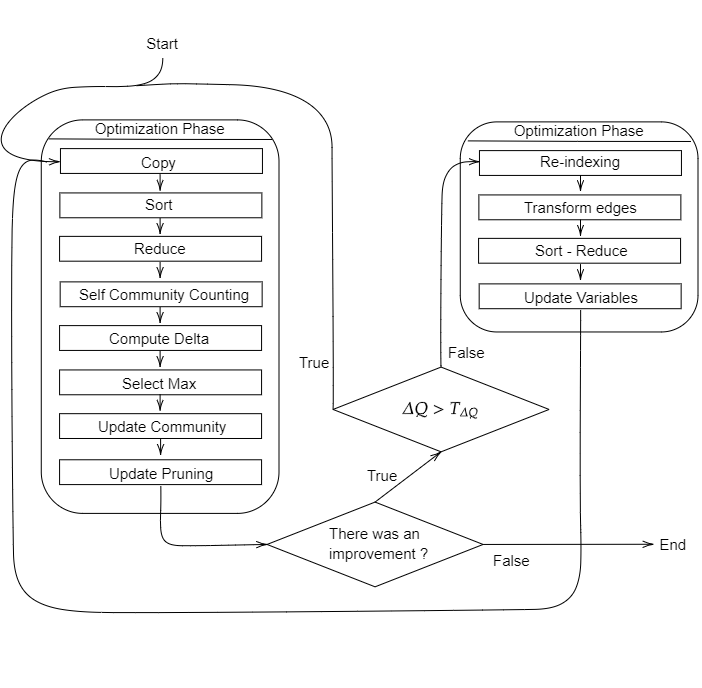
\includegraphics[width=1\linewidth]{0-resources/PSR-Louvain-Schema}
	\caption{Schema of the PSR-Louvain algorithm. At the beginning, we first execute the eight sub-phases that composed the optimization phase. After that, if there isn't an improvement respect the value of $Q$ that we have before the start of the first iteration of the optimization phase we stop the algorithm. Otherwise, we check if the current $\Delta Q$ is greater than a threshold: if this is true, we re-iterate the optimization phase, otherwise we execute the four sub-phases of the aggregation phase. After the optimization phase, we re-start from the optimization phase.}
	\label{fig:psr-louvain-schema}
\end{figure}

\begin{enumerate}
	\item \textbf{Copy sub-phase:}  this algorithm implements firstly the pruning presented by Ozaki in the parallel behaviour \cite{pruning}. Therefore, in the first step, we copy from the list of edges, all those that belongs to a node that we have consider in this iteration. To due this, we check on a support vector if the source nodes of the edges have a neighbour that has change community according to the criteria presented in Chapter \ref{prun}. We use a support vector to check if the node matched the requirement: in position $i$ there is a True if the nodes $i$ matched the criteria in the previous iteration, False otherwise. At the first iteration all the nodes are considered. We exclude from the copy also the self-loops because we don't consider them in the computation of the various values of $\Delta Q$. Besides, in this phase, we don't copy destination nodes $j$ but we substitute that values with the associated community $c_j$. Therefore, we obtain a list of tuples that contain the source node $i$, the community $c_j$ related to the linked node $j$ and the weight of the edge $w$.  
	
	\item \textbf{Sort sub-phase:} This algorithm uses a scheme of computation inspired by \cite{cheong2013hierarchical}. In the second phase, we sort the data obtained in the first phase. Given the list of tuples $(i, c_j, w)$ created in the previous sub-phase, we sort it using the pair $(i, c_j)$ as key.  At the end of this phase, we have that all the tuples $(i, c_j, w)$ with the same $(i, c_j)$ are consecutive. Besides, all the tuples with the same source node $i$ are consecutive.
	
	\item \textbf{Reduce sub-phase:} in this step we perform a reduction by key, i.e. we sum up all consecutive values with the same key. We use as key the tuple $(i, c_j)$: doing this, we obtain a unique tuple $(i, c_j,$  $l_{i\rightarrow c_j})$ for each pair $(i, c_j)$ where $l_{i\rightarrow c_j}$ is the sum of all the weights of edges that links the node $i$ with a node in the community $c_j$. We need this value to calculate later the $\Delta Q_{i\rightarrow c_j}$.
	
	\item \textbf{Self community counting  sub-phase:} In this phase, we isolate all the tuples  $(i, c_j, l_{i\rightarrow c_j})$ such that 
	$c_j$ is the actual community for the nodes $i$, i.e. $c_i$. We need to isolate these values $l_{i\rightarrow c_i}$ because we use it in the next phase to compute the various values of $\Delta Q$ (Eq. (\ref{delta_q})).
	
	\item \textbf{Compute Delta sub-phase:} Now we can calculate the $\Delta Q_{i\rightarrow c_j}$ for each tuple using the Eq. (\ref{delta_q}) , because we calculated all the $l_{i\rightarrow c_j}$ in the previous steps and we have the weights of the communities and the weights of the nodes in input. After the computation, we obtain a list of tuple $(i, c_j, \Delta Q_{i\rightarrow c})$.
	
	\item \textbf{Select Max sub-phase:} Now we need to isolate the maximum $\Delta Q_{n\rightarrow c_j}$ for each node $n$. Considering that the vector is already sorted, we can perform this operation using another reduction, but, in this case, we return only the maximum weight. We execute this operation using the nodes $i$ as keys.  After this step, we have exactly one tuple  $(i, c_z, \Delta Q_{i\rightarrow c_z})$  for each nodes $i$ where $c_z$ is the community that gives the maximum increase in modularity $\Delta Q_{i\rightarrow c_z}$ if the node $i$ is assigned to $j$.
	
	\item \textbf{Update Community sub-phase:}\label{update_com} In this step, we update the community for each node if the value of $\Delta Q_{i\rightarrow c_z}$ is greater than 0. We also update the related community weights: we remove the weight of the node from the previous community and we add it to the new one. These operations are implemented as atomic to avoid concurrent operations.  We also keep track if each node changed or not its community. We remark that this
	vector is different respect to the array that we use in the first step. In the following step, we create the pruning vector from this one.

	
	\item \textbf{Update Pruning sub-phase:}\label{update_prun} : To update the vector that handles the pruning
	criteria, we firstly set all its elements to zero. After that, a method takes each
	edge of the graph and check if the destination edge has changed its communities
	in the previous iteration: if this happened, the corresponding node value is set
	to True. This update operation is not atomic, because multiple threads can
	set only a True to the same position and there aren’t conflict.

\end{enumerate}
Afterwards, we compute the new modularity score and than we compare the obtained value with the old one: if the value is larger than a given threshold, we repeat these steps, otherwise we start the aggregation phase. We highlight that we can not add directly the various $\Delta Q$ obtained in the optimization step to the old modularity
like the sequential algorithm, because all nodes change communities simultaneously and consequently this value is not reliable any more.
The Algorithm \ref{alg:sort-optimization} summarize the phase.
\begin{algorithm}
	\caption{Prune-Sort-Reduce: Optimization phase}\label{alg:sort-optimization}
\begin{algorithmic}
\Procedure{optimizationPhase}{Graph $G$, Community $C$}
	\State $pruning = vector(True, n\_nodes)$
	\State $old\_delta = 0$
	\State $delta = modularity(G,C)$
	\While{ $delta - old\_delta <$ THRESHOLD}
		\State $node\_to\_community = \text{[ ]}$
		\State $self\_values = \text{[ ]}$
		\State $ $
		\Comment{copy}
		\For{\textbf{each} edge $(i,j,w)$ in $G$ \textbf{in parallel}}
			\If{$pruning[i]$ == $True$ and $i$ != $j$}
				\State $node\_community.append(i,C[j],w)$
			\EndIf
		\EndFor 
		\State $ $
		\Comment{sort}
		\State $node\_community.parallel\_sort(by= \text{source, community})$
		\State $ $
		\Comment{reduce}
		\State $node\_community.parallel\_reduce(\text{ }by= \text{source, community}, $
		\Statex[12] $operation= \text{sum})$
		\State $ $
		\Comment{self-counting}
		\For{\textbf{each} $(i,cj,l)$ in $node\_community$ \textbf{in parallel}}
		\If{$C(i)$ == $cj$}
			\State $self\_values[i] = l$
		\EndIf
		\EndFor
		\State $ $
		\Comment{delta}
		\State $s = size(node\_community)$
		\For{$z$ in $[0,1,...,s]$ \textbf{in parallel}}
			\State $node\_community[z] = compute\_delta(node\_community[z],$ 
			\Statex[14] $self\_values,$ 
			\Statex[14] $communities\_weight,$
			\Statex[14] $nodes\_weight)$
		\EndFor
		\State $ $
		\Comment{max}
		\State $node\_community.parallel\_reduce(\text{ }by= \text{source},$
		\Statex[9] $operation= \text{max})$
		\State $ $
		\Comment{update community}
		\State $is\_change = vector(False, n_nodes)$
		\For{\textbf{each} $(i, cz, delta)$ in node\_to\_community \textbf{in parallel}}
			\If{$delta > 0$}
				\State $atomicAdd(communites\_weight[C[i]], -nodes\_weight[i])$
				\State $atomicAdd(communites\_weight[cz], nodes\_weight[i])$
				\State $C[i] = cz$
				\State $is\_change[i] = True$
			\EndIf
		\EndFor
		\State $ $
		\Comment{update pruning}
		\For{\textbf{each} edge $(i,j,w)$ in $G$ \textbf{in parallel}}
			\If{$is\_change[j]$ == $True$}
				\State $pruning[i] = True$
			\EndIf
		\EndFor
		\State $old\_delta = delta$
		\State $delta = modularity(G,C)$
	\EndWhile
	\EndProcedure
	\end{algorithmic}
\end{algorithm}\newpage
\noindent The aggregation phase uses several similar concepts presented previously, and we can divide it into four sub-phases in which the operations are executed in parallel:
\begin{enumerate}
	\item \textbf{Re-indexing communities sub-phase:}\label{Re-indexing} in the first phase, before the graph contraction, we assign a new id to the communities. Actually, we have only certain communities associated to the nodes respect to the initial configuration: for example, if a nodes $i$ change community from $c_1$ to $c_2$ in the first iteration of the optimization phase, no nodes are assigned to $c_1$ after the update and no nodes can select the communities $c_1$ from that moment. This cause a useless waste of memory if we continue to keep all those unused values in the community weight. For this reason, we need to create a map to rearrange the communities index.
	First, we create a support vector such that at the position $c$ there is a 1 if the community $c$ has a weight greater than 0 (i.e. there is at least one node assigned to this community). Then we perform a prefix sum on this vector: in this way at the position $c$ there is the new index incremented by one for the community $c$ (please note: incremented by one because we counting from zero).
	 We remark that even if the empty communities are still mapped with this method and have the same indexes of the community at the preceding position respect them, we doesn't have any conflict because we doesn't use these entry.
	 When this renumbering map is ready, we start the next phase.
	\item \textbf{Transform edges sub-phase:} In this step, all the pairs of edges $(i, j)$ of the original graph are transformed in the pair $(c_i, c_j)$ where $c_i$ ($c_j$) is the community associated to $i$ ($j$). In this phase, we also apply the map to renumber the communities that we create in the previous step. 
	\item \textbf{Sort-Reduce sub-phase:} In this phase we sort all the edges $(c_i, c_j, w)$ using as a key for the sorting the pair $(c_i, c_j)$. After this, we reduce the edges vector still using as a key $(c_i, c_j)$. After this step we have contract the graph summing up all the edges that lay between two communities.
	\item \textbf{Update variables sub-phase:}\label{updategraph}  In the last step, we update all the support value in the graph object, like the number of the nodes, the number of edges, the nodes weights. We also reset the communities object reordering the communities weight according to the re-indexing map and assigning each node to a community composed only by itself.
\end{enumerate}
The Algorithm \ref{alg:sort-aggregation} summarizes this phase. 
The PSR-Louvain continues to alternate this two phases until we can not have further improvement in the modularity update. In this version of the algorithm, we keep only the best result to not occupy several device memory, but it is possible trivially save the intermediate result adding a step that save the clustering results after the re-indexing sub-phase (in this way we have consistent indexing among the dendrogram).
\begin{algorithm}
	\caption{Prune-Sort-Reduce: Aggregation phase}\label{alg:sort-aggregation}
	\begin{algorithmic}
		\Procedure{aggregationPhase}{Graph $G$, Community $C$}
		\State $ $
		\Comment{re-indexing}
		\For{$i$ in size($communities\_weight$) \textbf{in parallel}}
		\If{ $communities\_weight[i]$  == $0$)}
		\State $map[i] = 0$
		\Else
		\State $map[i] = 1$
		\EndIf
		\EndFor 
		\State $map.prefix\_sum()$
		\State $ $
		\Comment{transform}
			\For{\textbf{each} edge $(i,j,w)$ in $G$ \textbf{in parallel}}
			\State $\text{Substitute } i , j \text{ with } map[C[i]], map[C[j]]$
		\EndFor 
		\State $ $
		\Comment{sort-reduce}
		\State $G.edges.parallel\_sort(by= \text{"source, community"})$
		\State $G.edges.parallel\_reduce(by= \text{"source, community"}, $
		\Statex[9] $operation= \text{"sum"})$

		\State $ $
		\Comment{update}
		\State $G.update()$
		\State $C.update(G)$	
		\EndProcedure
	\end{algorithmic}
\end{algorithm}
\newpage
\subsection{PH-Louvain}
This second version of the parallel Louvain algorithm is quite similar to the previous:
it still has a pruning approach, but uses a different way to aggregate the weights of edges that link a node to the same community: we use a special global hashmap instead of sorted vector.
Using a map to accumulate some values by its key is a standard approach to solve this problem because the map allows to retrieve and insert an object in $O(1)$ time. 
To obtain this performance, the hashmap uses a function named hash function to dispose at random the objects in the memory. This creates a problem on the GPU because uncoalesced memory accesses is an order of magnitude slower than sequential memory accesses. 
To overcome this problem this map uses a system of open-addressing based on the cuckoo hashing: this type of map is the one that performs better on the GPUs \cite{alcantara2012building}, thanks to a simple and efficient management of the conflicts. This map uses 64 bits for the key and 32 bits for the value. We choose to use 64 bits for the key because we need to store a pair of 32 bits keys (the pair $(node, community)$ in the optimization phase and the $(community, community)$ pair in the aggregation phase). This map has $r$ different hash function, each one associated to an id $r_i$ where $i \in [0, r-1]$. When we insert a new pair key-value $(k,v)$, we use the hash function with id $r_0$ to compute the position of the new key $v$: if the slot is empty, we add the key and the value, we use the next function $r_1$ otherwise. We continue to search a empty slot following this schema: if $r_i$ is not empty, we retry to insert the pair with function $r_{i+1}$. If all the function fails to insert the new pair, we raise an error.\\ 
The main difference between this map and the classic cuckoo hashing is that 
the original version of the map when we try to insert an entry in a position that is already filled, the map remove the old pair key-value, insert the new one and try to find a new position for the old value using another hash function.  
In our map, we don't "kick out" the old key when we have a conflict in order to find a new memory address for it, but we hash with a different function the pair that we have to insert: this because to make a classic cuckoo hashing, we need a set of atomic operations for 128bits to do the "kick out" operation in parallel without generating race condition. This type of atomic operation in CUDA can be done only on variable up to 64 bits. Besides, this map has another special feature: if we insert a pair $(k,v)$ and there is already an entry in the table with a key $k$, the map automatically sum the values $v$ to the one stored in the map. Indeed, we use this map only to aggregate values, and for this reason, we design it to perform this operation as fast as possible. The last feature that we add to this table is the contract table operation: this methods transform the map in a pair of contiguous vector re-arranging the memory, in order to allow us to access to each pair key-value sequentially. After this operation, we can not get the entry using the hash function, because the memory is re-organized. We use this operation before the computation of $\Delta Q$ to increase the performance and still working considering the edges $(nodes, communities)$ independently. 
\begin{figure}[t!]
	\centering
	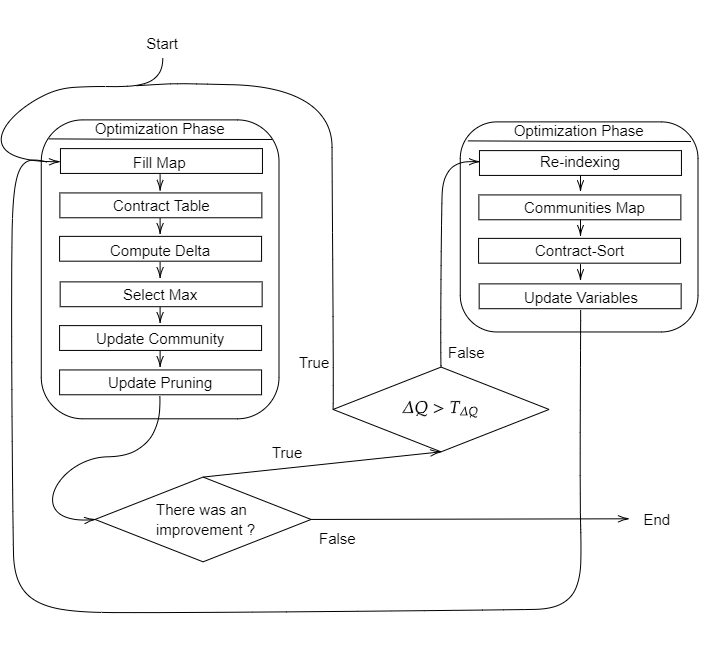
\includegraphics[width=1\linewidth]{0-resources/PH-Louvain}
	\caption{Schema of the PH-Louvain algorithm. At the beginning, we first execute the six sub-phases that composed the optimization phase. After that, if there isn't an improvement respect the value of $Q$ that we have before the start of the first iteration of the optimization phase we stop the algorithm. Otherwise, we check if the current $\Delta Q$ is greater than a threshold: if this is true, we re-iterate the optimization phase, otherwise we execute the four sub-phases of the aggregation phase. After the optimization phase, we re-start from the optimization phase.}
	\label{fig:ph-louvain}
\end{figure}
Now we present the algorithm. At the start of the optimization phase we have each edge represented as a tuple $(i,j,w)$,  a the weight of each node,  a map that associates each nodes with the corresponding communities  and the the total weight of each communities like the previous algorithm. 
We divide the optimization phase into six sub-phases:
\begin{enumerate}
	\item \textbf{Fill Map sub-phase:} in the first step, for each edge $(i,j,w)$, we insert into the map the tuple $(n, c_j, w)$ where $c_j$ is the community associated to the destination node $j$. We use as a key the pair $(n,c_j)$.
	We consider only the tuple that has the source node that matching the criteria presented in \\Chapter \ref{prun}. We use a support vector identical to the one presented in the previous algorithm. We also exclude all the self-loops in this phase. At the end of this step we obtain a map where every non-empty entry has the form $(i, c_i, l_{i \rightarrow c_j})$. The map also isolate in a different vector each value $l_{i \rightarrow c_i}$ such that $c_i$ is the community of the node $i$. Each value  $l_{i \rightarrow c_i}$ is stored at position $i$. This operation was made because in the delta step, after the contraction, we can not get any more the position of the entry using the hash function, and we need a method to get the nodes communities weights quickly. 
	
	\item \textbf{Contract Table sub-phase:} in the first step, using a map to calculate $l_{i \rightarrow c_j}$ allows accessing to the memory address in $O(1)$ time for each edge. But to compute the relative delta and the maximum, we obtain better performance if we access to the memory using an uncoalesced memory access pattern. In addition, we have no idea of how and which community are in the neighbourhood of a given node. One alternative may be to allocate a thread for each edge, each thread transforms the edge destination from nodes to community, gets the consequent pair from the map and then check the maximum. This approach lay to check multiple time the score of the community $c$ if two neighbours of the nodes $n$ are in $c$. To overcome this problem, we contract the table: the vector that composed the table are re-organized in order to permit sequential access, without empty slots between the entries. After this operation, the map becomes a vector containing the tuples $(i, c_j,l_{i \rightarrow c_j})$. The support vector with the sum of edges of the node that connects it with another in the same community is not re-arranged by this operation.
	
	\item \textbf{Compute Delta sub-phase:} now we can compute the $\Delta Q_{i\rightarrow c_j}$ for each tuple $(i, c_j, l_{i \rightarrow c_j})$ using the Equation \ref{delta_q}. The result overwrites the last value in the tuple (we doesn't need that value any more). To get the sum of edges that connect the nodes to its actual community, we use the vector created in the first step.
	
	\item \textbf{Select Max sub-phase:} now we have a vector of tuple $(i, c_j, \Delta Q_{i\rightarrow c_j})$. Now we have to select the pair $(c_i, \Delta Q_{i\rightarrow c_j})$ for each node $i$ such that $\Delta Q_{i\rightarrow c_j}$ is maximum. We can not use as the previous algorithm a reduce operation because we haven't a sorted array and the sorting operation is too expansive. Instead, for each tuple, we check if the value $\Delta Q_{i\rightarrow c_j}$ is greater compered to the one of the tuple saved in a support array at the position $i$: if it is, we substitute the old value with the new one, we do nothing otherwise. To avoid race condition in the insert, these operation are executed atomically. At the end of this step, we have exactly one tuple $(i, c_z, \Delta Q_{n\rightarrow c_x)}$ for each node $i$, like the previous algorithm.
	
	
	\item \textbf{Update Community sub-phase:} This phase update the community just like the one presented in the Prune-Sort-Reduce version (\ref{Prune-Sort-Reduce}, optimization sub-phase \ref{update_com}).
	
	\item \textbf{Update Pruning sub-phase:} This phase create the array with the pruning information just like the one presented in the Prune-Sort-Reduce version (\ref{Prune-Sort-Reduce}, optimization sub-phase \ref{update_prun}).
\end{enumerate}
The Algorithm \ref{alg:hash-optimization} summarizes this phase.
\begin{algorithm}
	\caption{Hashmap: Optimization phase}\label{alg:hash-optimization}
	\begin{algorithmic}
		\Procedure{optimizationPhase}{Graph $G$, Community $C$}
		\State $pruning = vector(True, n\_nodes)$
		\State $old\_delta = 0$
		\State $delta = modularity(G,C)$
		\State $ $
		\While{ $delta - old\_delta <$ THRESHOLD}
		\State $ $
		\Comment{fill map}
		\For{\textbf{each} edge $(i,j,w)$ in $G$ \textbf{in parallel}}
		\If{$pruning[i]$ == $True$ and $i$ != $j$}
		\State $hashmap.insert(i,C[j],w)$
		\EndIf
		\EndFor 
		\Comment{contract}
		\State $list = hashmap.contract()$
		\State $ $
		\Comment{delta}
		\For{$z$ in size(list) \textbf{in parallel}}
		\State $list[z] = compute\_delta(list[z], hashmap.self\_values,$ 
		\Statex[10] $communities\_weight, nodes\_weight)$
		\EndFor
		\State $ $
		\Comment{max}
		\State $result = \text{[ ]}$
		\For{\textbf{each} $(i, cj, delta)$ in list \textbf{in parallel}}
		\State $\text{START OF THE ATOMIC BLOCK} $
		\State $(i, cj_{old}, delta_{old}) = result[z]$
		\If{$delta > delta_{old}$}
		\State $result[z] = (i, cj, delta)$ 
		\EndIf
		\State $\text{END OF THE ATOMIC BLOCK} $
		\EndFor
		\State $list = result$
		\State $ $
		\Comment{update community}
		\State $is\_change = vector(False, n_nodes)$
		\For{\textbf{each} $(i, cz, delta)$ in list \textbf{in parallel}}
		\If{$delta > 0$}
		\State $atomicAdd(communites\_weight[C[i]], -nodes\_weight[i])$
		\State $atomicAdd(communites\_weight[cz], nodes\_weight[i])$
		\State $C[i] = cz$
		\State $is\_change[i] = True$
		\EndIf
		\EndFor
		\State $ $
		\Comment{update pruning}
		\For{\textbf{each} edge $(i,j,w)$ in $G$ \textbf{in parallel}}
		\If{$is\_change[j]$ == $True$}
		\State $pruning[i] = True$
		\EndIf
		\EndFor
		\State $ $
		\State $old\_delta = delta$
		\State $delta = modularity(G,C)$
		\EndWhile
		\EndProcedure
	\end{algorithmic}
\end{algorithm}
\newpage
\noindent
We continue to execute this step until the difference in modularity between the configuration drops below a given threshold. The consideration of the computing of $\Delta Q$ in parallel behaviour presented in the previous chapter is still valid. 
The aggregation phase of this algorithm use once again the map to aggregate, but the key in this context is composed of $(community_{source}, community_{destination})$. We can divide this phase in four sub-phase like the previous version:
\begin{enumerate}
	\item \textbf{Re-indexing communities sub-phase:} In this sub-phase we associate each community to a new id to reduce the waste of memory. This sub-phase is identical to the sub-phase with the one with the same name presented in the PSR-Louvain description (\ref{Prune-Sort-Reduce}, aggregation sub-phase \ref{Re-indexing}). 
	\item \textbf{Communities map sub-phase:} In this step, all the tuple of edges $(i, j, w)$ of the original graph are inserted in a hash table. Before the insertion, we transform each entry in the tuple $(r_i, r_j, w)$ where $r_i$ is an index of the community associated with $i$ after the remapping. We use as key the pair $(r_i, r_j)$. At the end of this step, we have each edge of the new graph, because we sum up all the edges that lay between two communities.
	\item \textbf{Contract-sort sub-phase:} At the beginning of this phase, we have a map containing all the edges of the new graph. However, the graph object store the edges information using three ordered vectors, so we have to re-organize the information stored in the unordered and uncoalesced map. To do this, we use the contract operation to transform the map in a vector of tuple $(c_i, c_j, tot)$ and then we sort the arrays according to the order of the first one. Finally, we have the updated graph.
	\item \textbf{Update variables sub-phase:} This phase update the new graph and the related communities object just like the one presented in the Prune-Sort-Reduce version (\ref{Prune-Sort-Reduce}, aggregation sub-phase \ref{updategraph}).
\end{enumerate}
The Algorithm \ref{alg:hash-aggregation} summarize this phase. 
Like the previous algorithm, this one continues to alternate the two main phases until no further improvement in the modularity update can be obtained.
\begin{algorithm}
	\caption{Hashmap: Aggregation phase}\label{alg:hash-aggregation}
	\begin{algorithmic}
		\Procedure{aggregationPhase}{Graph $G$, Community $C$}
		\State $ $
		\Comment{re-indexing}
		\For{$i$ in size($communities\_weight$) \textbf{in parallel}}
		\If{ $communities\_weight[i]$  == $0$)}
		\State $map[i] = 0$
		\Else
		\State $map[i] = 1$
		\EndIf
		\EndFor 
		\State $map.prefix\_sum()$
		\State $ $
		
		\Comment{map}
		\For{\textbf{each} edge $(i,j,w)$ in $G$ \textbf{in parallel}}
			\State $hashmap.insert(map[C[i]],map[C[j]],w)$
		\EndFor 
		
		\State $ $
		\Comment{contract-sort}
		\State $G.edges = hashmap.contract()$
		\State $G.edges.parallel\_sort(by= \text{"source, community"})$
		\State 
		
		\State $ $
		\Comment{update}
		\State $G.update()$
		\State $C.update(G)$
		
		\EndProcedure
	\end{algorithmic}
\end{algorithm}

\subsection{Speed-up the First Iteration in the Optimization Phase}\label{f-1}
In this chapter, we present an optimization technique that we add into our code to speed-up the first iteration of each optimization phase. We include this method in both versions of the algorithm presented previously. We focus this presentation on the Prune-Sort-Reduce version, even if the concept that allows us to optimize the algorithm is still present in the Hashmap version. At the beginning and also after each aggregation phase, we notice that we have a configuration in which each node is assigned to each self-community, i.e., each node $i$ is assigned to the community $c_i$ and it is the only node assigned to it. In this configuration, when in the copy sub-phase we transform each edge $(i,j)$ in the pair $(i,c_j)$ where $c_j$ is the community of the node $j$, we obtain the same original pair, because the index of $c_j$ is equal to $j$. In addition, considering that each node is assigned to a different community, we don't need the sort and reduce sub-phases, because the pairs $(i, j)$ are already sorted by the construction of the graph object (we need a sorted vector for the select max sub-phase) and the reduction is useless, because all the pairs have a different composite key $(i, j)$.
Also the self-counting sub-phase is useless, because no edge that isn't a self-loop lay  nodes in the same community and during the copy sub-phase we excluding the self-loop from the computation. 
Considering all these facts, we choose to remove in the first iteration this three sub-phases and also to avoid the useless transformation in the copy sub-phase. For the Hashmap version of the algorithm, we still use this optimization based on the other version because we use the hashmap to aggregate different edges and this aggregation is no longer necessary.

\subsection{Data structure and implementation details}\label{impl-details}
The two main structures that we need to represent are the original graph and the community structure. Commonly a graph $G(V, E)$ is represented using its adjacency matrix: each node is associated with an incremental id in the range $(0, n-1)$ where $n$ is the number of nodes. To retrieve the weights of an edge between two nodes, we look to the values stored at the position $(id_1, id_2)$. As we say in the chapter \ref{3.1}, the community detection techniques are effective if executed on sparse graphs.  Therefore, if we use a matrix to represent a sparse graph, this matrix will have a lot of zeros. Even if this pattern allows to retrieve the weight of an edge in constant time, this data structure isn't suitable for a problem that involves millions of data because we need too much memory to allocate this matrix and it has several unused values. Therefore, we have the necessity of compress the adjacency matrix. To do this, we choose to represent it using a coordinate list (often referred to as COO). We have three vectors \verb|edges_source|,  \verb|edges_destination| and  \verb|weights| that contain respectively the ids of the rows, the ids of the columns and the values. The standard modularity optimization is computed on undirected graphs: this means that the adjacency matrix is symmetric and we can store in the COO list only the upper triangle of the matrix and we still have all the edges represented. Despite this observation, we store all the values of the adjacency matrix because we need those repeated values in these algorithms when we transform the destination node in the destination community. These vectors are also sorted by the pair $(source, destination)$ and there is a vector named  \verb|neighboorhood_sum| of length $n$ in which at position $i$ there is the starting position of the edges that have source $i$ in \verb|edge_source|. Thanks to this vector, we can retrieve fast all the neighbour of a given node. These particular COO lists are also known as compressed neighbour lists. In the graph object, we also store a vector named \verb| tot_weight_per_nodes| that associate each node $i$ to its degree, the total degree of the graph, the number of nodes and the number of the edges. We use \verb|thrust::device_vector| to store all this data on the GPUs memory. In summary, the graph object is the following:
\begin{lstlisting}[language=C++]
struct GraphDevice {
	unsigned int n_nodes;
	unsigned long n_links;
	double total_weight;

	thrust::device_vector<unsigned> tot_weight_per_nodes;
	thrust::device_vector<unsigned int> neighbourhood_sum;

	thrust::device_vector<unsigned int> edge_source;
	thrust::device_vector<unsigned int> edge_destination;
	thrust::device_vector<unsigned int> weights;
}
\end{lstlisting}
We design the community object so that it contains the graph associated with it. We notice that the maximum number of different communities is pair to the total number of nodes: this is also the configuration at the beginning of the algorithm. Considering this, we choose to identify each community with an incremental id in the range $(0, n-1)$, like we do previously with the nodes. Therefore, in the community object, we have a vector named \verb|communities| of length $n$ in which in the position $i$ there is the id of the community of the node $i$. Besides, there is a vector of size $n$ that associate each community to its total weight.  In summary,  the community object is the following:
\begin{lstlisting}[language=C++]
struct Community {
	GraphDevice graph;
	
	thrust::device_vector<unsigned int> communities;
	thrust::device_vector<double> communities_weight;
}
\end{lstlisting}
After the initial parsing, we use only the device memory to store the data. The GPU memory is related to the machine and it is usually smaller than a RAM.
To reduce the memory used simultaneously during the optimization phase, the Prune-Sort-Reduce algorithm divides the edges in buckets of fixed size. 
The algorithm executes the sub-phases from the first to sixth on a bucket, stores the results and start the execution on another bucket. When all buckets are considered, we execute the last two updating sub-phases. This reduce the required memory used to store the data from $2*m$ (used to store two vector that can store all the nodes: one for the copy and one to store the reduced values) to $2*size(bucket) + n$ (two vector of the bucket size for the copy and the reduce operation and a vector to store the best result for each node). 
In order to compute the right maximum values of $\Delta Q$ for each node, we split the edges into buckets such that if there is an edge with source node n in the bucket, also all the other edges that belong to n are included. To perform this, we use the \verb|neighbourhood_sum| vector to select the right range. The Hashmap version implements a similar logic, performing repeatedly the first four sub-phases on different buckets,  and then eventually update the communities and the pruning vector when all buckets are processed. We use buckets of maximum size equals to 50 000 000.

Both algorithms implements also the minimum label heuristic (Chapter \ref{parallel-imp}): we change communities only if the id of the new communities is lower than the old one for communities composed only by a single node to prevent the simultaneous swap. We also select the communities with the lowest id when we have multiple communities with the greatest $\Delta Q$ for the same node: this method leads to a faster convergence.

In the algorithms, each parallel sub-phase presented for both algorithm takes as an input a list of element on which execute its computation, and we assign to each thread one of this element in our kernels. We also use the \verb|thrust| library to perform the sorting, the transforming, the reducing and the prefix sum operations. When we need to consider the edges vector as a unique tuple, we use a \verb|zip_iterator| to handle the data correctly.
The hashmap is stored in the device global memory and it is composed by two \verb|thrust::device_vector|: the first one, used for the keys, contains a \verb|unsigned long long|; the second one \verb|float|, used for the value, contains \verb|float|. We choose to use a \verb|unsigned long long| because in this way we can perform atomic operation on the composite key. The contract table operation is made quickly using the function \verb|thrust::remove_if| that removes from the vector every element $x$ that satisfies a predicate and then contract the vector. The predicate that we use check if the memory slot in the vectors is empty. 


In the Select max sub-phases of the Hashmap version, to avoid race condition caused by the two atomic operation that we have using considering independently each community $c$ and the associated $\Delta Q_{i\rightarrow c}$ (\verb|atomicMax| on the value and possibly \verb|atomicCAS| (compare and swap) for the associated community), in the implementation we transform this of 32 bits variable in a unique word of 64 bit. The half most significant bytes are filled by the value, the other part by the community. Thanks to this, we can consider it as a \verb|unsigned long long| and we can use an unique atomicMax to substitute both the values. 
